\documentclass[11pt,letterpaper]{article}
\usepackage[lmargin=1in,rmargin=1in,tmargin=1in,bmargin=1in]{geometry}
\usepackage{../style/homework}
\usepackage{../style/commands}
\setbool{quotetype}{true} % True: Side; False: Under
\setbool{hideans}{true} % Student: True; Instructor: False

% -------------------
% Content
% -------------------
\begin{document}

\homework{7: Due 10/13}{The only function of economic forecasting is to make astrology look respectable.}{John Galbraith}

% Problem 1
\problem{10} As accurately as possible and showing all your work, find the least square regression line, along with the $r$ and $r^2$ value, for the dataset $\{ (1, 0), (0, 1), (1, 1), (2, 6) \}$. Show all your work. 



\newpage



% Problem 2
\problem{10} Given the following information below, find the least square regression line. Show all your work. 
	\[
	\begin{aligned}
	n&= 10 &&& R&= -0.0023 \\
	\overline{x}&= 0.97 &&& \quad s_x^2&= 30.32 \\
	\overline{y}&= -1.33 &&& \quad s_y^2&= 36.54
	\end{aligned}
	\]



\newpage



% Problem 3
\problem{10} Match each regression coefficient to its corresponding graph. 
	\begin{figure}[!ht]
	\centering
	\begin{minipage}{0.45\textwidth}
	   \centering
	   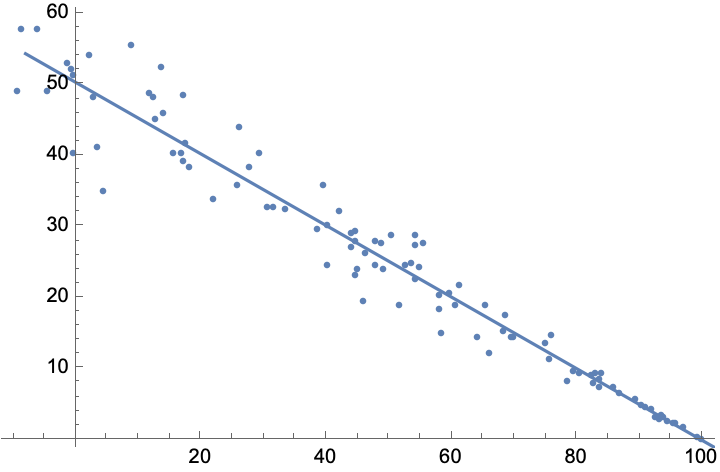
\includegraphics[width=0.9\textwidth]{reg1.png}
	   \caption*{(a)}
	\end{minipage}\hfill
	\begin{minipage}{0.45\textwidth}
	   \centering
	   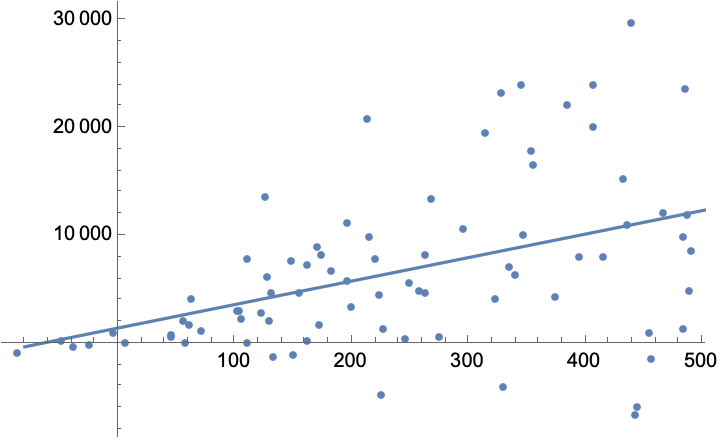
\includegraphics[width=0.9\textwidth]{reg2.png}
	   \caption*{(b)}
	\end{minipage}
	\begin{minipage}{0.45\textwidth}
	   \centering
	   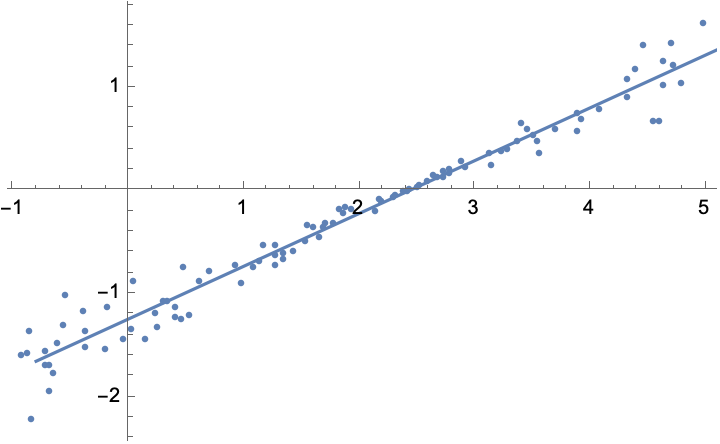
\includegraphics[width=0.9\textwidth]{reg3.png}
	   \caption*{(c)}
	\end{minipage}
	\begin{minipage}{0.45\textwidth}
	   \centering
	   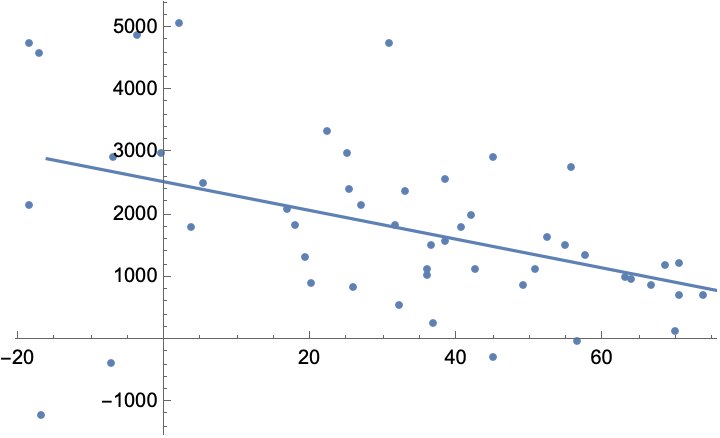
\includegraphics[width=0.9\textwidth]{reg4.png}
	   \caption*{(d)}
	\end{minipage}
	\end{figure}

\begin{enumerate}[(i)]
\item \underline{\hspace{1.5cm}}: $R= -0.9725$
\item \underline{\hspace{1.5cm}}: $R= -0.4639$
\item \underline{\hspace{1.5cm}}: $R= 0.4337$
\item\underline{\hspace{1.5cm}}: $R= 0.9826$
\end{enumerate} 



\newpage



% Problem 4
\problem{10} A researcher is predicting penguin weights given their final adult height. The create a linear regression model for the weight of the penguin (in lbs), $W$, given its heigh in cm, $h$. Their model is $W(h)= 0.8h - 56.2$.
	\begin{enumerate}[(a)]
	\item What are $b_0$ and $b_1$ for this linear regression?
	\item How much does a penguin's weight increase per centimeter taller that it is, according to this model?
	\item Does the $y$-intercept for this model hold any meaning? Explain. 
	\item Predict a penguin's weight if its height is 125~cm. Suppose one of the penguins in their dataset has a height of 125~cm and weight of 48.6~lbs. Find the residual for this datapoint. 
	\item The researcher finds an $R^2$ value of $0.4329$. Is this linear model a good predictor of a penguin's weight given its height? Explain. 
	\end{enumerate}


\end{document}